\section{Our Approach}
%Briefly introduce the whole framework, and refer to each subsection one by one.
%In this section, we describe the details about how we add the loss,
%which significantly increases the quality of relation extraction results.
%In this section, we describe a novel loss term that incorporates the type constraints and the cardinality constraints required by each relation,
%which significantly increases the quality of relation extraction results.
First, we briefly introduce our base relation extraction model, 
then we describe our constraints in detail and how to incorporate these constraints during training.
%Before delving into the details of our method (Sec.~\ref{sec:loss_term}), we first briefly introduce our base relation extraction model (Sec.~\ref{sec:base_model}), and the constraints that we will use (Sec.~\ref{sec:constraints}).




\subsection{Base Model}
\label{sec:base_model}
%Briefly introduce the base model (PCNN).
While our method is adapted to most existing relation extractors, in this paper, we take the attentive convolutional neural network~\cite{lin2016neural} as our base model, which is currently one of the most widely used extractor in \RE.
It operates in the \MIL framework, specifically
%that takes in a \textbf{\emph{sentence bag}} and outputs the relations between these two entities.
%that takes in all the sentences mentioning the target subject and object, and output the relations between these two entities.
it uses convolutional neural network for sentence embedding, and an attention layer to selectively aggregate sentence embeddings into a sentence bag embedding, which is then fed to a softmax classifier to generate the predicted relation distribution. 
%\red{(YY: I changed the $\bm{p}$ to $\bm{r}$, because the SL equation has $\bm{p}$)}


%Specifically, \APCNN operates in the \MIL framework that takes in all the sentences mentioning the target subject and object, and output the relations between these two entities.
%We first use the piecewise convolutional neural network (\PCNN)~\cite{zeng2015distant} to obtain the embedding of each sentence.
%Then, an attention layer is applied to these sentence embeddings to selectively aggregate them into a sentence bag embedding, which is then fed to a softmax classifier to generate the predicted relation distribution, $\bm{p}$.

%First, we concatenate the word embeddings and position embeddings of each word in one sentence, the position embeddings indicates how close each word is to head or tail entities. Then, we use a convolutional layer with window size 3, a max pooling layer and a non-linear layer to merge all these features and get the representation of one sentence.Then a selective attention is done over a bag of sentences to get the bag representation.


\subsection{Relation Constraints}
\label{sec:constraints}
%Describe clw's argument type constraints

%\cite{xu2017semantic}  encodes the symbolic knowledge in Boolean logic, and derives a semantic loss to make the neural network automatically learn the symbolic knowledge. Their experiments show that the semantic loss helps to reduce the constraint violation and gives significant practical improvements in semi-supervised classification. 

%Inspired by their work, we encode the constraints in \cite{chen2014encoding} to boolean logic, and add a semantic loss to the neural network.

Our relation constraints are similar to those used by  Chen et al.~\shortcite{chen2014encoding}.
Specially,
%Following Chen et al.~\shortcite{chen2014encoding}, 
our relation constraints are defined over each combination of two entity pairs:$(subj_1, r_1, obj_1)$ and $(subj_2,  r_2, obj_2)$
(we use $subj$, $obj$ and $r$ to denote subject, object and relation for entity pair, respectively, in the rest of the paper).
We derive type constraints and cardinality constraints from existing KB to implicitly capture the expected type and cardinality requirements for the arguments of a relation.
%details see Chen et al.~\shortcite{chen2014encoding}. 
%\red{(YY: add the cite)}
%\paragraph{Implicit Argument Types Inconsistencies:}
\paragraph{Type Constraint}
%Due to the lack of well-defined typing systems in most \KBs, determining the expected argument type of each relation with appropriate granularity is usually a hard problem.
%Generally, the argument types of the correct predictions should be consistent with each other.
%Similar to Chen et al.~\shortcite{chen2014encoding}, we also use entity sharing between relations to implicitly capture the expected argument type of each relation.
If the subject (or object) set of relation $r_1$ in \KB has a large intersection with those of $r_2$, then we consider $r_1$ and $r_2$ to have the same expected subject (or object) type.
We thereby assign relation pairs ($r_1$, $r_2$) into $\bm{C}^{ts}$ (or $\bm{C}^{to}$) if they have the same subject (or object) type,
% $\bm{C}^{to}$ if they have the same object type, 
$\bm{C}^{tso}$  if the subject type of one relation is the same as the object type of the other.
%We thereby collect relation pairs that have the same subject type ($\bm{C}^{ts}$), object type ($\bm{C}^{to}$), 
%and similarly, relation pairs where the subject type of one relation is the same as the object type of the other ($\bm{C}^{tso}$).
%and similarly, relation pairs whose subject type of $r_1$ is the same as the object type of $r_2$ ($\bm{C}^{tso}$).
%finding relation pairs that can share the same subject ($C^s$), object ($C^o$), and those where the subject of one relation can be the object of the other ($C^{so}$).
%Then, $\bm{C}^{ts}$, $\bm{C}^{to}$ and $\bm{C}^{tso}$ represents the constraints that we expect ($r_1$, $r_2$) of each combination of ($subj_1$, $r_1$, $obj_1$) and ($subj_2$, $r_2$, $obj_2$) to fall into $\bm{C}^{ts}$ when $subj_1=subj_2$, $\bm{C}^{to}$ when $obj_1=obj_2$ and $\bm{C}^{tso}$ when when $subj_1=obj_2$ or $subj_2=obj_1$, respectively.
%Then, we expect the relations of all pairs of predicted \emph{(subject, relation, object)} triples to fall into $\bm{C}^{ts}$, $\bm{C}^{to}$ or $\bm{C}^{tso}$ when they share the same entity in either subject or object.
The idea is that, if the predicted relations of two triples require the same entity to belong to different types, then at least one of the prediction must be wrong.
%The idea is that, take $C^s$ for example, if the subject set of relation $R_1$ has a large intersection with those in $R_2$ (($R_1$, $R_2$) lies in $C^s$ ), then the expected subject type of $R_1$ and $R_2$ are likely to be the same. Therefore, if a pair of predicted relation $R_1'$ and $R_2'$ for two entity pairs share the same subject, which implies $R_1'$ and $R_2'$ have the same expected subject type, then ($R_1'$, $R_2'$) must lie in $C^s$. 
%\red{luo: Hard to explain this clearly given limited space. Maybe we can delete the intuition part.}

% if the predicted relations of two entity pairs require the same entity to belong to mutually-exclusive types, then at least one of the prediction must be wrong.
%Take \textless USA, New York\textgreater and \textless USA, Washington D.C.\textgreater as an example. We couldn't predict two relations for them which has different Subject types, such as $ LargestCity $ and $ LocationCity $.

%\paragraph{Violations of Arguments' Uniqueness:}
\paragraph{Cardinality Constraint}
Given a subject (or object), some relations should have only one object (or subject).
For example, the relation \emph{Capital} would expect only one object for a given subject.
Following this observation, we assign relation $r$ into $\bm{C}^{cs}$ (or $\bm{C}^{co}$) if it can have multiple subjects (or objects) for a given object (or subject).
%$\bm{C}^{co}$ if it can have multiple objects for a given subject.
%Following this observation, we collect relations that can have multiple objects ($\bm{C}^{co}$) or subjects ($\bm{C}^{cs}$).
%Then, $\bm{C}^{co}$ (or $\bm{C}^{cs}$) represents the constraints that we expect the relation $r$ of each combination of ($subj_1$, $r$, $obj_1$) and ($subj_2$, $r$, $obj_2$), which have the same relation $r$, to fall into $\bm{C}^{co}$ (or $\bm{C}^{cs}$) when $subj_1=subj_2 \land obj_1\neq obj_2$ (or when $subj_1\neq subj_2 \land obj_1=obj_2$)
%expect the predicted relations that have multiple objects (or subjects) for a given subject (or object) to fall into $\bm{C}^{co}$ (or $\bm{C}^{cs}$).

% For example, given USA as the subject of the relation Capital, we can only accept one possible object, because there is great chance that a country only have one capital.

%Subj-Cons: $r_1$ and $r_2$ can't have same subject. Obj-Cons means $r_1$ and $r_2$ can't have same object. Subj-Obj-Cons means $r_1$'s subject can't be $r_2$'s object or $r_2$'s subject can't be $r_1$'s object. Subj-Uni means if $r_1$ equals $r_2$, 

Thus we finally get 5 sub-category constraint sets $\bm{C^{\Phi}}$, where $\bm{\Phi}=\{ts, to, tso, cs, co\}$

\subsection{Incorporate  Constraints for Training}
\label{sec:loss_term}
In this section, we demonstrate our method of converting the relation constraints into a loss using the Semantic Loss framework~\cite{xu2017semantic}.
We also introduce a variant of our method to speed up the training process by sampling some constraints.

\paragraph{Relation Constraint Loss}
%Describe semantic loss, and how to encode clw's constraints into semantic loss.
Semantic loss is a general framework that can encode propositional logic constraints as a loss in a principled way.
%and derive a semantic loss to make the neural network automatically learning the symbolic knowledge. 
%This loss function captures how close the neural network is to satisfying the constraints on its output. 
Concretely, the semantic loss is defined as:
%For example, the semantic loss between an exactly-one constraint $\alpha$ and a neural net output vector $p$ captures how close the prediction $p$ is to having exactly one output set to true(1), and all false(0), regardless of which output is correct.
%We desire our semantic loss $L^{s}(\alpha, p)$ to be proportional to the negative log-probability of $\alpha$ being satisfied when sampling values according to $p$. More formally,
%In \cite{xu2017semantic}, the semantic loss function is formed as follows,
%\begin{small}
\begin{equation}
\label{seq:semantic_loss}
	L^{s}(\bm{C}, \bm{p}) = -log\sum\limits_{\bm x\models\bm{C}}\prod\limits_{i:\bm x\models X_i}p_i\prod\limits_{i:\bm x\models \neg X_i}(1-p_i)
\end{equation}
%\end{small}
%over variables $\bm X=\{X_1,...,X_n\}$, and a vector of probabilities $p$, where $p_i$ denotes the predicted probability of variable $X_i$: 
where $\bm{C}$ is a set of constraints defined over variables $\bm{X}=\{X_1,...,X_n\}$, 
$p_i$ is the predicted probability of $X_i$,
specifically $X_i$ corresponds a single relation and $p_i$ is defined in Eq.~(\ref{Eq:compute_p}) in our work.
$\bm x \models \bm{C}$ refers to the assignment $\bm{x} = \{x_1,...,x_n\}$ of variables $\bm X$ that satisfies the constraints in $\bm{C}$,
and $i\colon\bm x \models X_i$ (or $i\colon\bm x\models \neg X_i$) refers to the indices $i$ where $x_i$ is set to true (or false) in assignment $\bm x$.

%As for our type constraints, the variables $\bm{X}\in \{0,1\}^{2R}$, where $R$ is the number of relations,
%are defined over a pair of  relations ($r_1$, $r_2$) that are assigned to 2 entity pairs ($subj_1$, $obj_1$) and ($subj_2$, $obj_2$) respectively.
%Specifically, $X_i\in \bm{X}_{1...R}$ equals 1 only when $r_1$ is the $i^{th}$ relation,
%and $X_{R+i}\in \bm{X}_{R+1...2R}$ equals 1 only when $r_2$ is the $i^{th}$ relation.
%We thereby define three semantic loss terms: $m^{ts}L^{s}(\bm{C}^{ts}, \bm{p})$, $m^{to}L^{s}(\bm{C}^{to}, \bm{p})$, $m^{tso}L^{s}(\bm{C}^{tso}, \bm{p})$, where $m^{ts}$, $m^{to}$, $m^{tso}$ are 0-1 masks that are set to 1 when $subj_1=subj_2$, $obj_1=obj_2$, $subj_1=obj_2$ respectively.
%\red{(YY: version of type constraints)}

As for our type constraints, the assignment $\bm x$ of variables $\bm{X}\in \{0,1\}^{R}$, where $R$ is the number of relations, 
is derived by a pair of relations $(r_1, r_2) \in \bm{C}^{ts} \cup \bm{C}^{to} \cup \bm{C}^{tso}$. 
%Specifically, $X_i, X_j\in \bm{X}_{1...R}, i\neq j$ equals 1 only when $r_1$ is the $i^{th}$ relation, and $r_2$ is the $j^{th}$ relation.
Specifically, $x_i\in \bm{x}$ equals 1 only when $r_1$ or $r_2$ is the $i^{th}$ relation,
and all $x_i\in \bm{x}$ are set to 0 when $r_1=r_2$.

As for our cardinality constraints, the assignment $\bm x$ of variables $\bm{X}\in \{0,1\}^{R}$ is derived by one relation $r \in \bm{C}^{cs} \cup \bm{C}^{co}$. 
Specifically, $x_i\in \bm{x}$ equals 1 only when $r$ is the $i^{th}$ relation.

\iffalse
%We thereby define two semantic loss terms: $m^{co}L^{s}(\bm{C}^{co}, \bm{p})$ and $m^{cs}L^{s}(\bm{C}^{cs}, \bm{p})$, where $m^{co}$ and $m^{cs}$are 0-1 masks that are set to 1 %when $subj_1=subj_2 \land obj_1\neq obj_2$ and $subj_1\neq subj_2 \land obj_1=obj_2$ respectively.

%We thereby define three semantic loss terms: $m^{ts}L^{s}(\bm{C}^{ts}, \bm{p})$, $m^{to}L^{s}(\bm{C}^{to}, \bm{p})$, $m^{tso}L^{s}(\bm{C}^{tso}, \bm{p})$, over 2 entity pairs %($subj_1$, $obj_1$) and ($subj_2$, $obj_2$), where $m^{ts}$, $m^{to}$, $m^{tso}$ are 0-1 masks that are set to 1 when $subj_1=subj_2$, $obj_1=obj_2$, $subj_{1(or\;2)}=obj_{2(or\;1)}$ %respectively.

%As for our type constraints, the variables $\bm{X}\in \{0,1\}^{R}$, where $R$ is the number of relations,
%are defined over a pair of relations ($r_1$, $r_2$) that are assigned to 2 entity pairs ($subj_1$, $obj_1$) and ($subj_2$, $obj_2$) respectively.
%Specifically, $X_i, X_j\in \bm{X}_{1...R}, i\neq j$ equals 1 only when $r_1$ is the $i^{th}$ relation, and $r_2$ is the $j^{th}$ relation.
%Specifically, $X_i\in \bm{X}$ equals 1 only when $r_1$ or $r_2$ is the $i^{th}$ relation,
%and all $X_i\in \bm{X}$ are set to 0 when $r_1=r_2$.
%We thereby define three semantic loss terms: $m^{ts}L^{s}(\bm{C}^{ts}, \bm{p})$, $m^{to}L^{s}(\bm{C}^{to}, \bm{p})$, $m^{tso}L^{s}(\bm{C}^{tso}, \bm{p})$, where $m^{ts}$, $m^{to}$, $m^{tso}$ are 0-1 masks that are set to 1 when $subj_1=subj_2$, $obj_1=obj_2$, $subj_{1(or\;2)}=obj_{2(or\;1)}$ respectively.
%means that $X_i$ is set to true in world $\bm x$. 
%Intuitively, this is the self-information of obtaining an assignment that satisfies the constraint. 
%Intuitively, utilizing this loss pushes up the likelihood of assignments $\bm x$ that satisfies sentence $\alpha$.

%As for our cardinality constraints, the variables $\bm{X}\in \{0,1\}^{R}$ are defined over a relation $r$ that is assigned to ($subj_1$, $obj_1$) and ($subj_2$, $obj_2$) simultaneously.
%Specifically, $X_i\in \bm{X}$ equals 1 only when $r$ is the $i^{th}$ relation,
%We thereby define two semantic loss terms: $m^{co}L^{s}(\bm{C}^{co}, \bm{p})$ and $m^{cs}L^{s}(\bm{C}^{cs}, \bm{p})$, where $m^{co}$ and $m^{cs}$are 0-1 masks that are set to 1 %when $subj_1=subj_2 \land obj_1\neq obj_2$ and $subj_1\neq subj_2 \land obj_1=obj_2$ respectively.

%Note that, for each loss term, all the relation assignment pairs that satisfies the corresponding constraints are included.
%Therefore, minimizing these semantic loss terms actually increases the likelihood of all the relation predictions that satisfies our relation constraints.
\fi

%To utilize \cite{chen2014encoding}'s constraints into our neural net, we transform these constraints into boolean logic just like \cite{xu2017semantic}. For example, (Subj, Obj, Subj-Obj, rel1, rel2) = (1, 0, 0, Nationality, Birthplace) is a constraint in \cite{chen2014encoding}, limiting the argument type of relations, which means that two relation $ Nationality $ and $ Birthplace $ could have the same Subject , different Object and one relation's Subject is different with other's Object. Suppose there are 5 kinds of relations: rel1, rel2=$ Nationality $, rel3, rel4=$ Birthplace $, rel5, we encode this rule with a boolean vector (1, 0, 0, 0, 1, 0, 1, 0), the first three position indicates the (Subj, Obj, Subj-Obj) information, and the last five position indicates which two relations involved in the rule. And all the boolean form of constraints in \cite{chen2014encoding} composed of  $ \alpha $ in (1).

\paragraph{Training Procedure}
%How do you construct the batches?
%What is the loss function?
Here we introduce the learning and optimization details of our model. Our objective function consists of two parts:
\begin{equation}
	J(\theta) = J_{en}(\theta) + J_{SL}(\theta)
\end{equation}
where  $J_{en}(\theta)$ is the original cross-entropy classification loss, and $J_{SL}(\theta)$ is our semantic loss.

%The cross-entropy loss defined as follows:
%\begin{equation}
%	J_{en}(\theta)= \sum\limits_{i=1}^{s}logp(r_i|S_i, \theta)
%\end{equation}
%where $ s $ indicates the number of sentence bags and $ \theta $ indicates all parameters of our model.

%For any combination of two entity pair in a batch, we use the outputs of our base model to get the probability vector $\bm{p}$ in Eq.~\ref{seq:semantic_loss},
%and thereby compute the semantic loss terms $m^{*}L^{s}(\bm{C}^{*}, \bm{p})$.
%Here $m^{*}L^{s}(\bm{C}^{*}, \bm{p})$ denotes the sum of all the semantic loss terms defined in Sec.~\ref{sec:loss_term}.

For any combination of two entity pairs in a batch, we use $\bm{p}_{ij}^{t}$ and $\bm{p}_{ij}^{c}$ in Eq.~(\ref{Eq:compute_p}) to denote the probability vector $\bm{p}$ for type and cardinality constraints in Eq.~(\ref{seq:semantic_loss}), respectively.
\begin{equation}
\label{Eq:compute_p}
%\bm{p}_{i} = \bm{p'}_{1i} + \bm{p'}_{2i} - \bm{p'}_{1i}*\bm{p'}_{2i};\;\; \bm{p}_{i} = \bm{p'}_{1i}*\bm{p'}_{2i}
\bm{p}_{ij}^{t} = 1-(1-\bm{p'}_{i})(1-\bm{p'}_{j});\;\; \bm{p}_{ij}^{c} = \bm{p'}_{i}\bm{p'}_{j}
\end{equation}
where $\bm{p'}_i$ and $\bm{p'}_j$ represents the relation distribution outputs of our base model for the two entity pairs,
$\bm{p}_{ij}^{t}(t \in \{ts, to, tso\})$ and $\bm{p}_{ij}^{c}(c \in \{cs, co\})$ denotes the predicted probability of variables $\bm{X}$ in the type and cardinality constraints, respectively.

And then we compute the semantic loss terms $\lambda ^{k}m^{k}L^{s}(\bm{C}^{k}, \bm{p}_{ij}^{k}), (k \in \bm{\Phi})$ for each sub-category constraints over two entity pairs.
%($subj_1$, $obj_1$), ($subj_2$, $obj_2$).
Here $\lambda^{k}$ denotes the corresponding weight coefficient and $m^{k}$ is a 0-1 mask which is set to 1 when the two entity pairs satisfies the conditions of $\bm{C}^{k}$.
%Then we use Eq.~\ref{seq:semantic_loss} to calculate $L^{s}(\alpha, p)$ on all combinations of two entity pair.

We demonstrate the calculating process of $L^{s}(\bm{C}^{to}, \bm{p}_{ij}^{to})$ in Fig.~\ref{fig:example}, where two entity pairs are (Bard College, New York) and (AT\&T, New York), satisfy the conditions having the same object type of $\bm{C}^{to}$.

\begin{figure}[h]
	\centering
	\begin{minipage}[t]{0.5\textwidth}
		\centering
		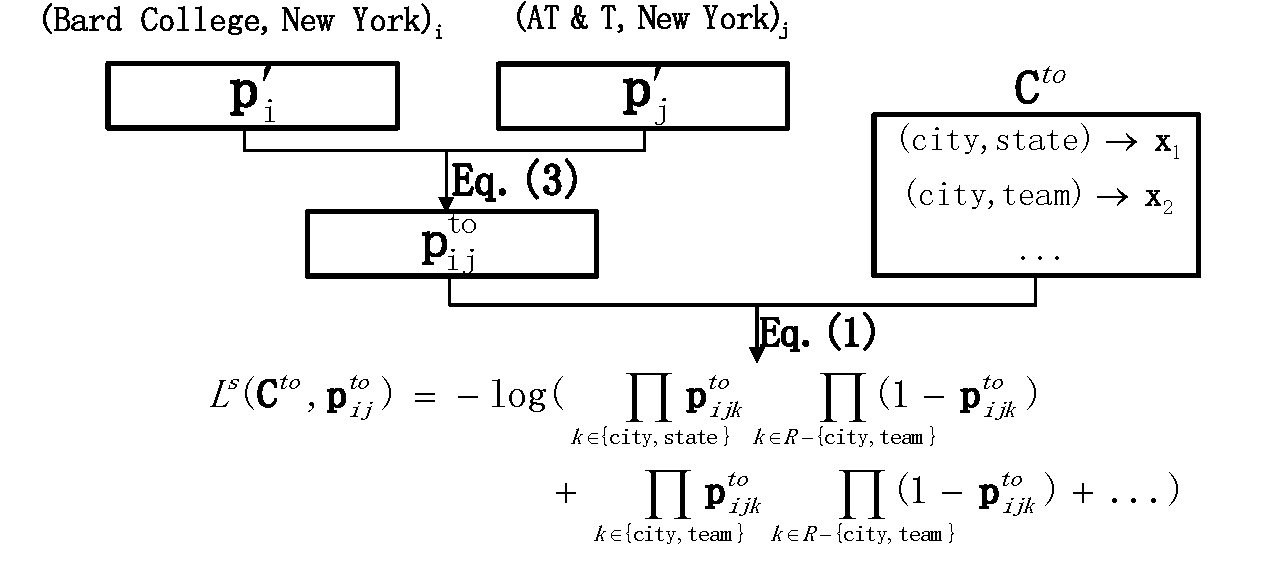
\includegraphics[width=8cm]{./result-figure/example.pdf}
		\caption{Calculate example}
		\label{fig:example}
	\end{minipage}
\end{figure}

Finally our semantic loss is defined as follows:
\begin{equation}
	%J_{SL}(\theta) = \sum\limits_{i < j}{\lambda ^{*}m^{*}L^{s}(\bm{C}^{*}, \bm{p}_{ij})}
	J_{SL}(\theta) = \sum\limits_{i < j}{\sum_{k\in \bm{\Phi}}{\lambda ^{k}m^{k}L^{s}(\bm{C}^{k}, \bm{p}_{ij}^{k})}}
\end{equation}
where $0\leq i < j < batch\_size$,
$\bm{p}_{ij}^{k} $ refers to the probability vector generated from Eq.~(\ref{Eq:compute_p}).

Note that, for each loss term, all the relation assignment pairs that satisfies the corresponding constraints are included.
Therefore, minimizing these semantic loss terms actually increases the likelihood of all the relation predictions that satisfies our relation constraints.

During training, we iterate by randomly selecting a mini-batch from the training set until converge, and adopt the Adam optimizer~\cite{kingma2014adam} to minimize the objective function.
% To solve the optimization problem, we adopt Adam \cite{kingma2014adam} to minimize the objective function. For learning, we iterate by randomly selecting a mini-batch from the training set until converge.
\paragraph{Simplified Semantic Loss}
In Eq.~(\ref{seq:semantic_loss}), for each entity pair combination, we need to calculate the semantic loss for every $\bm x \models \bm{C}$, which would be time-consuming since there are many relation assignments that are consistent with the constraint set $\bm{C}$.
However, among these assignments, only the gold standard relation assignment is the one that we desire.
Therefore, we simplifies Eq.~(\ref{seq:semantic_loss}) by only including the gold relation assignment and a few randomly sampled consistent assignments as supplements.
With this simplification, we wish to speed up the training process with only minor drop in performance.


%we find that for each entity pair combination, there exists $ \bm x $ that is more important than others

%Describe the simplified version of the semantic loss.
%In our experiments, we find that the way \cite{xu2017semantic} calculating semantic loss is time-consuming, so we simplify the semantic loss calculation without losing much performance, which greatly reduces the time overhead.

%In (1), we need calculate semantic loss for every $ \bm x (\bm x \models \alpha)$, but we find that for each entity pair combination, there exists $ \bm x $ that is more important than others. So we use the gold information of entity pairs to find the most important positive rule, and random sample some rules as a supplement. This significantly reduces the computational complexity.

